%% =====================================================================
%%   Stochastic ODE-Guard  ---  IEEE TNNLS submission (May 2026)
%%   Initial double-anonymous version per IEEE Author Portal policy.
%%   Compile with: pdflatex -> bibtex (or rerun pdflatex 3x for inline bib)
%%   Target: 10 pages two-column journal layout (max 15 with $200/page fee)
%% =====================================================================

%% --- For initial double-anonymous submission to TNNLS:
\documentclass[journal,10pt]{IEEEtran}
%% --- For camera-ready (after acceptance), switch to:
%% \documentclass[journal]{IEEEtran}
%% --- NOTE: do NOT use [compsoc] -- TNNLS is a CIS journal, not Computer Society.

%% --- Packages ------------------------------------------------------
\usepackage[utf8]{inputenc}
\usepackage[T1]{fontenc}
\usepackage{amsmath,amssymb,amsthm,amsfonts,mathtools}
\usepackage{bm}
\usepackage{algorithm,algorithmic}
\usepackage{booktabs}
\usepackage{multirow,makecell}
\usepackage{graphicx}
\usepackage{subcaption}
\usepackage{tikz}
\usepackage{pgfplots}
\pgfplotsset{compat=1.18}
\usetikzlibrary{arrows.meta,positioning,fit,backgrounds,calc,shapes.geometric,decorations.pathreplacing}
\usepackage[hyphens]{url}
\usepackage[hidelinks]{hyperref}
\usepackage{cleveref}

%% --- Theorem environments per IEEE Editorial Style Manual -----------
\newtheorem{theorem}{Theorem}
\newtheorem{lemma}[theorem]{Lemma}
\newtheorem{proposition}[theorem]{Proposition}
\newtheorem{corollary}[theorem]{Corollary}
\theoremstyle{definition}
\newtheorem{definition}[theorem]{Definition}
\newtheorem{assumption}[theorem]{Assumption}
\theoremstyle{remark}
\newtheorem{remark}[theorem]{Remark}

%% --- Notation ------------------------------------------------------
\newcommand{\Real}{\mathbb{R}}
\newcommand{\Exp}{\mathbb{E}}
\newcommand{\Prob}{\mathbb{P}}
\newcommand{\Var}{\mathrm{Var}}
\newcommand{\KL}{\mathrm{KL}}
\newcommand{\Lip}{\mathrm{Lip}}
\newcommand{\Brn}{\mathrm{B}}
\newcommand{\Fcal}{\mathcal{F}}
\newcommand{\Gcal}{\mathcal{G}}
\newcommand{\Xcal}{\mathcal{X}}
\newcommand{\Ycal}{\mathcal{Y}}
\newcommand{\Hcal}{\mathcal{H}}
\newcommand{\Ncal}{\mathcal{N}}
\newcommand{\Acal}{\mathcal{A}}
\newcommand{\Dcal}{\mathcal{D}}
\newcommand{\Lcal}{\mathcal{L}}
\newcommand{\Zcal}{\mathcal{Z}}

\begin{document}

%% =====================================================================
%%  TITLE  (anonymous version for initial submission)
%% =====================================================================
\title{Stochastic ODE-Guard: A Neural Stochastic Differential Equation
       Framework with Anti-Concentration Bounds for Adversarially Robust
       Network Intrusion Detection}

%% --- Anonymous author block for IEEE double-anonymous review ------
\author{
  \IEEEauthorblockN{Anonymous Authors}\\
  \IEEEauthorblockA{Submitted to \emph{IEEE Transactions on Neural Networks
   and Learning Systems}\\Double-anonymous initial submission, May 2026}
}

%% --- Camera-ready author block (commented out until acceptance) ----
%% \author{R.~N.~Anaedevha,~\IEEEmembership{Student~Member,~IEEE,}
%%         A.~G.~Trofimov,
%%     and Y.~V.~Borodachev
%% \thanks{R.~N.~Anaedevha, A.~G.~Trofimov, and Y.~V.~Borodachev are with
%%  the Institute of Cyber Intelligence Systems, National Research Nuclear
%%  University MEPhI (Moscow Engineering Physics Institute), 31~Kashirskoe
%%  Highway, 115409 Moscow, Russia.
%%  E-mail: ar006@campus.mephi.ru. ORCID:
%%  R.\,N.\,Anaedevha~\href{https://orcid.org/0000-0000-0000-0000}{0000-0000-0000-0000}.
%%  Manuscript received May~17, 2026.}}

\markboth{IEEE Transactions on Neural Networks and Learning Systems, Vol.~XX, No.~Y, May~2026}%
{Anonymous \MakeLowercase{\textit{et al.}}: Stochastic ODE-Guard}

\maketitle

%% =====================================================================
%%  ABSTRACT  (target 200--250 words, single paragraph)
%% =====================================================================
\begin{abstract}
Adversarially robust network intrusion detection remains an open problem
because per-flow neural classifiers degrade catastrophically under
small adversarial perturbations that nevertheless preserve the
underlying packet semantics. Existing certified defences such as
Lipschitz-bounded networks and randomised smoothing trade clean accuracy
against certificate radius and rarely transfer to the long-tailed,
high-dimensional feature spaces that production intrusion detection
and prevention systems must handle. We introduce \textbf{Stochastic
ODE-Guard}, a neural stochastic differential equation framework that
treats flow embeddings as the terminal state of an It\^o diffusion whose
drift and diffusion coefficients are jointly learned. The framework
admits three theoretical guarantees: a marginal-coverage property
on the terminal-state classification head, a Bismut--Elworthy--Li
identity that yields stable gradient estimators for the diffusion
parameters, and---as our principal original contribution---a
\emph{probabilistic robustness proposition} that follows from the
Carbery--Wright anti-concentration inequality applied to the
Wiener-chaos expansion of the smoothed score. Empirical validation
uses three Kaggle-released benchmark suites (ICS3D cloud security,
IIS3D integrating UNSW-NB15, CIC-IDS2018 and CIC-IoT-2023, and an
encrypted-and-post-quantum-cryptography traffic corpus) totalling
$1.84{\times}10^{7}$ flows, alongside the deployed open-source
RobustIDPS.ai platform whose registry of fourteen detectors provides
the comparison baselines. Stochastic ODE-Guard achieves $96.4\%$ clean
F1 and $93.1\%$ F1 under PGD-40 at $\epsilon{=}0.03$, exceeding the
strongest deployed baseline (SDE-TGNN, $96.0\%$ clean / $87.2\%$ adversarial)
while maintaining $1.7$~ms median inference latency. Comparison against
eight academic, commercial, and LLM-safety baselines shows
Stochastic ODE-Guard occupies the Pareto frontier on the clean-accuracy
vs.\ certified-radius plane.
\end{abstract}

%% --- Index Terms (4-5 alphabetical, period-terminated) -------------
\begin{IEEEkeywords}
Adversarial robustness, anti-concentration inequalities, network intrusion
detection, neural stochastic differential equations, uncertainty
quantification.
\end{IEEEkeywords}

%% =====================================================================
\section{Introduction}\label{sec:intro}
%% =====================================================================
\IEEEPARstart{N}{etwork} intrusion detection and prevention systems
(IDPS) have become the principal line of defence against the
escalating volume of cyber-physical threats targeting cloud,
edge, and Internet-of-Things deployments. Modern neural IDPS deliver
clean-traffic F1 scores exceeding $0.97$ on canonical benchmarks
such as UNSW-NB15 and CIC-IDS2017~\cite{wu2022rtids,halbouni2022cnnlstm},
yet these same models routinely lose more than fifteen F1 points under
projected-gradient adversarial perturbations whose $\ell_\infty$
budget is too small to alter the semantics of the underlying
flow~\cite{ennaji2024advsurvey,vitorino2024advbench}. The vulnerability
is not merely academic: structural adversarial attacks on
graph-neural-network IDPS have already been demonstrated to evade
production-grade detectors at line rate~\cite{venturi2024structural}.

The dominant certified-robustness strategies---Lipschitz-bounded
networks~\cite{tsuzuku2018lipschitz,anil2019sorting,araujo2023sll}
and randomised smoothing~\cite{cohen2019smoothing,salman2019smoothadv,yang2020smoothing}---deliver
formal guarantees but suffer two structural limitations
when transplanted into IDPS. First, Lipschitz certificates degrade
linearly with input dimension, which is punishing for the
$83$-dimensional flow vectors produced by modern feature
extractors~\cite{anil2019sorting}. Second, randomised smoothing
inflates inference latency by the Monte-Carlo sample budget required
for tight Clopper--Pearson certificates, which is incompatible with
the sub-millisecond per-flow envelope of production
sensors~\cite{cohen2019smoothing}. Both families also assume the
classifier is a deterministic map, ignoring the natural stochasticity
of continuous-time network dynamics.

A complementary line of work has shown that continuous-time neural
dynamics---neural ordinary differential equations
(NODEs)~\cite{kang2021sodef,guglielmi2025minimal}---inherit beneficial
robustness from the Gr\"onwall--Bellman inequality on their flow map.
Extending the framework from NODEs to neural stochastic differential
equations (NSDEs)~\cite{tzen2019nsde,li2020scalable,kidger2021nsdegan}
introduces an explicit diffusion term whose role under adversarial
perturbation has, until now, been left implicit. Recently the
\emph{stable Neural SDE} family~\cite{oh2024stablesde} established
existence and uniqueness conditions on the irregular-time-series
setting, and applications to graph uncertainty~\cite{bergna2024lgnsde}
confirm that the diffusion channel carries calibrated epistemic
information. What has been missing is a tractable robustness theory
that links the SDE diffusion coefficient to a finite-sample
adversarial certificate.

This paper closes that gap. We introduce \textbf{Stochastic ODE-Guard},
a neural stochastic differential equation framework whose drift and
diffusion are jointly learned on flow features, whose gradients are
estimated through a Bismut--Elworthy--Li
identity~\cite{bismut1981martingales,elworthy1994formulae}, and whose
adversarial robustness derives from an anti-concentration argument on
the Wiener-chaos expansion of the smoothed score. The framework was
prototyped inside the deployed \texttt{RobustIDPS.ai} open-source
platform whose registry of fourteen detectors provides both
infrastructure and competitive baselines, and was validated on three
Kaggle-released benchmark suites totalling $1.84\times 10^7$ flows.

We make four contributions, each tied to the section that develops it.

\emph{(C1) An anti-concentration probabilistic robustness proposition.}
Section~\ref{sec:theory} establishes that the gap between the smoothed
score at a clean input and at an adversarial perturbation is
anti-concentrated in the sense of Carbery and
Wright~\cite{carbery2001anticonc}. The bound is polynomial in the
perturbation budget and explicitly identifies the degree of the
Wiener-chaos expansion as the controlling parameter. To our knowledge
this is the first robustness certificate that follows from the
algebraic structure of the diffusion (rather than from Lipschitz
contraction or Gaussian-noise smoothing).

\emph{(C2) A Bismut--Elworthy--Li gradient estimator for diffusion
parameters.} Section~\ref{sec:framework} derives the gradient of the
expected loss with respect to the diffusion coefficient using the
Bismut--Elworthy--Li (BEL)
formula~\cite{bismut1981martingales,elworthy1994formulae,hsu2002}.
The estimator is unbiased, has bounded variance under mild ellipticity,
and combines with the stochastic-adjoint sensitivity
method of Li \textit{et~al.}~\cite{li2020scalable} to give an
end-to-end trainable pipeline.

\emph{(C3) An integrated ablation across three Kaggle benchmarks and
the deployed platform.} Section~\ref{sec:exp} reports the first
unified evaluation of Stochastic ODE-Guard against the seven
\texttt{RobustIDPS.ai} detectors and four external academic baselines
on ICS3D~\cite{ds_ics3d}, IIS3D~\cite{ds_iis3d}, and the encrypted
post-quantum-cryptography (PQC) traffic corpus~\cite{ds_pqcids}.
The ablation isolates the contribution of (i)~the diffusion channel,
(ii)~the BEL gradient estimator, and (iii)~the anti-concentration
regulariser.

\emph{(C4) A Pareto-frontier comparison with current industry-grade
IDPS.} Section~\ref{sec:exp} situates Stochastic ODE-Guard against
eight contemporary baselines spanning academic neural IDPS
(E-GraphSAGE~\cite{lo2022egraphsage}, RTIDS~\cite{wu2022rtids},
IDS-GraphMamba~\cite{mosaiyebzadeh2025graphmamba}, and the deployed
SDE-TGNN), commercial signature engines
(Snort~3~\cite{snort3}, Suricata~7~\cite{suricata7}, Zeek~7~\cite{zeek7}),
and the LLM-safety filter Llama Guard~3~\cite{llamaguard3}.

The remainder is organised as follows. Section~\ref{sec:related}
surveys related work in four threads. Section~\ref{sec:prelim} states
the mathematical preliminaries that the rest of the paper builds upon.
Section~\ref{sec:framework} presents the Stochastic ODE-Guard
architecture and training procedure. Section~\ref{sec:theory} proves
the principal anti-concentration robustness result.
Section~\ref{sec:exp} reports the experimental setup, the integrated
ablation, and the industry comparison. Section~\ref{sec:disc}
discusses limitations and threats to validity, and
Section~\ref{sec:conc} concludes.

For readers approaching this work from a security-engineering rather
than a machine-learning background, the central conceptual move can be
summarised informally as follows. A network flow is a sequence of
packet-level statistics that a deployed sensor extracts in real time.
A classical neural classifier treats this flow as a single fixed
vector and predicts a label deterministically. Stochastic ODE-Guard
instead treats the flow as the starting point of a small random walk
in feature space and predicts the label by averaging over the walk's
endpoints. The random walk is governed by two learned components: a
\emph{drift} that pushes the state in the direction the data suggest,
and a \emph{diffusion} that adds calibrated noise. The diffusion is
what gives the framework its adversarial robustness, because a
small perturbation of the input has limited ability to move the
average endpoint when the endpoint is itself a noisy average.
The theoretical contribution quantifies exactly how limited that
ability is.

%% =====================================================================
\section{Related Work}\label{sec:related}
%% =====================================================================
Four bodies of literature converge on this work, and we organise our
discussion around them with the goal of positioning the contribution
that Section~\ref{sec:framework} will develop.

\emph{Certified adversarial robustness.} The Lipschitz-bounded family
established by Tsuzuku \textit{et~al.}~\cite{tsuzuku2018lipschitz}
and refined by Anil \textit{et~al.}'s GroupSort~\cite{anil2019sorting},
Wang and Manchester's Lipschitz-bounded deep
networks~\cite{wang2023lbdn}, and Araujo \textit{et~al.}'s SLL
parameterisation~\cite{araujo2023sll}, provides certificates whose
radius scales as the inverse network-Lipschitz constant. Randomised
smoothing~\cite{cohen2019smoothing} and its anisotropic
extensions~\cite{yang2020smoothing,eiras2022ancer} convert
non-robust base classifiers into smoothed classifiers with high-
probability $\ell_2$ certificates. PixelDP~\cite{lecuyer2019pixeldp}
established the differential-privacy connection that grounds the
Gaussian-smoothing analysis.
Section~\ref{sec:theory} contributes a fundamentally different
certificate which is neither Lipschitz nor smoothing-based: it
exploits the anti-concentration of polynomial chaos induced by the
SDE diffusion. The closest neighbour theoretically is the
Carbery--Wright bound~\cite{carbery2001anticonc} as developed by
Meka, Nguyen, and Vu~\cite{meka2016anticonc}, but neither was
previously applied to deep-learning robustness.

\emph{Neural ODEs and SDEs for robustness.} Kang \textit{et~al.}'s
SODEF~\cite{kang2021sodef} showed that Lyapunov-stable equilibrium
points in a neural ODE confer adversarial
robustness. Guglielmi \textit{et~al.}~\cite{guglielmi2025minimal}
quantified the minimal weight perturbation under which a neural ODE
loses robustness. Stable Neural
SDEs~\cite{oh2024stablesde} established well-posed extensions to
irregular time series, while Bergna \textit{et~al.}'s latent graph
neural SDE~\cite{bergna2024lgnsde} carried these ideas into the graph
setting. The stochastic-adjoint sensitivity method of
Li \textit{et~al.}~\cite{li2020scalable} provided the practical
training algorithm. Our work treats the diffusion as a robustness
mechanism rather than a generative-modelling tool (the latter is
the focus of score-based SDEs~\cite{song2021score}) and derives
a non-trivial certificate from its algebraic structure.

\emph{Network intrusion detection.} Lo \textit{et~al.}'s
E-GraphSAGE~\cite{lo2022egraphsage} brought edge-feature graph
neural networks to NIDS. Wu \textit{et~al.}'s
RTIDS~\cite{wu2022rtids} adapted the transformer to encrypted-flow
classification. Halbouni \textit{et~al.}'s hybrid
CNN-LSTM~\cite{halbouni2022cnnlstm} established the spatio-temporal
template subsequently refined by Mosaiyebzadeh \textit{et~al.}'s
IDS-GraphMamba~\cite{mosaiyebzadeh2025graphmamba}. Our previous work
contributed three building blocks to this line: a temporal-adaptive
neural ODE with deep spatio-temporal point processes for real-time
NIDS~\cite{anaedevha2026ode}, a stochastic multimodal transformer with
uncertainty quantification~\cite{anaedevha2025stochtx}, and a
robust-adversarial defence formulation~\cite{anaedevha2024ram}.
Earlier still, we examined device-identification baselines on
wireless intrusion traffic~\cite{anaedevha2024elcon}.

\emph{Stochastic neural networks and uncertainty.} The Bayesian
neural network literature beginning with
MacKay~\cite{mackay1992bnn} and extended in the adversarial setting by
Liu \textit{et~al.}'s Adv-BNN~\cite{liu2019advbnn} demonstrated that
posterior weight uncertainty confers some adversarial robustness, an
effect quantified by He \textit{et~al.}'s parametric noise
injection~\cite{he2019pni}. The PAC-Bayes
school~\cite{mcallester1999pacbayes,dziugaite2017pacbayes,perezortiz2021pacbayes}
provides generalisation certificates for stochastic networks that
we use in Section~\ref{sec:theory} as a complement to the
anti-concentration argument. Our prior work on MambaShield extended
selective state-space modelling to the poisoning-resilient
setting~\cite{anaedevha2026mambashield}, and our work on
uncertainty-calibrated hierarchical Gaussian processes furnished the
multi-scale temporal calibration we adopt here in
Section~\ref{subsec:training}~\cite{anaedevha2026uchgp}.

%% =====================================================================
\section{Mathematical Preliminaries}\label{sec:prelim}
%% =====================================================================
We collect the four classical results that underpin
Sections~\ref{sec:framework} and~\ref{sec:theory}, in each case
stating the conditions under which the result applies to our setting.
Throughout this paper, $\Real^d$ denotes the $d$-dimensional Euclidean
space, $W=(W_t)_{t\geq 0}$ denotes an $m$-dimensional standard Brownian
motion (the canonical mathematical model of accumulated Gaussian noise
across continuous time) on a filtered probability space
$(\Omega,\Fcal,\{\Fcal_t\}_{t\geq 0},\Prob)$ satisfying the usual
conditions, where $\Omega$ is the sample space of all possible noise
realisations, $\Fcal$ is the $\sigma$-algebra of measurable events,
$\{\Fcal_t\}$ is the filtration encoding information available up to
time $t$, and $\Prob$ is the underlying probability measure. The norm
$\|\cdot\|$ denotes the Euclidean norm and $I_d$ the
$d\times d$ identity matrix. The notation $A\succeq B$ for symmetric
matrices means $A-B$ is positive semi-definite. The expectation
$\Exp[\,\cdot\,]$ is taken over all Brownian sources unless an
explicit conditioning is shown. A reader who treats $W_t$ informally
as ``cumulative random kicks up to time $t$'' will not lose the
substance of any result below.

\subsection{Neural Stochastic Differential Equations}\label{subsec:nsde}
A neural stochastic differential equation on the time interval
$[0,T]$ is the It\^o SDE
\begin{equation}\label{eq:nsde}
  dX_t = f_\theta(X_t,t)\,dt + g_\theta(X_t,t)\,dW_t,\qquad X_0=x_0,
\end{equation}
where the drift $f_\theta:\Real^d\!\times\![0,T]\!\to\!\Real^d$ and the
diffusion $g_\theta:\Real^d\!\times\![0,T]\!\to\!\Real^{d\times m}$
are neural networks parameterised by $\theta$.

\begin{theorem}[Existence and uniqueness; {\protect\cite[Thm.~5.2.1]{oksendal2003}}]\label{thm:eu}
Assume the drift $f_\theta$ and the diffusion $g_\theta$ are
Borel-measurable and satisfy, uniformly in $t\in[0,T]$, the linear-
growth condition
$\|f_\theta(x,t)\|+\|g_\theta(x,t)\|\leq C(1+\|x\|)$
and the Lipschitz condition
$\|f_\theta(x,t)-f_\theta(y,t)\|+\|g_\theta(x,t)-g_\theta(y,t)\|\leq C\|x-y\|$
for some constant $C>0$. If the initial condition $X_0$ is independent
of $\sigma(W_s:s\geq 0)$ and satisfies $\Exp\|X_0\|^2<\infty$, then
\eqref{eq:nsde} admits a unique $\Fcal_t$-adapted strong solution
$X=(X_t)_{t\in[0,T]}$ with
$\Exp\!\int_0^T\!\|X_t\|^2\,dt<\infty$.
\end{theorem}

In practice the linear-growth and Lipschitz conditions are enforced by
spectral-normalisation of the neural-network weights of $f_\theta$ and
$g_\theta$ during training, exactly as in Anil \textit{et~al.}'s
GroupSort architecture~\cite{anil2019sorting}; we verify this
empirically in Section~\ref{sec:exp}.

\subsection{Bismut--Elworthy--Li Gradient Identity}\label{subsec:bel}
The BEL formula~\cite{bismut1981martingales,elworthy1994formulae,hsu2002}
expresses the gradient of an expectation under an SDE as a
Malliavin-weighted expectation of the integrand itself. It is the
mechanism by which gradients with respect to the diffusion
coefficient can be estimated without differentiating through a noise
realisation.

\begin{theorem}[Bismut--Elworthy--Li]\label{thm:bel}
Let $f\in C^2_b(\Real^d,\Real^d)$ and $g\in C^2_b(\Real^d,\Real^{d\times d})$
with $gg^\top(x)\succeq\lambda I_d$ uniformly for some $\lambda>0$
(uniform ellipticity, ensuring the noise has full-rank diffusion in
every direction), and let $X^x$ solve
$dX_t=f(X_t)\,dt+g(X_t)\,dW_t$, $X_0=x$. Let $J^x_t=\partial X^x_t/\partial x$
denote the first-variation process---the Jacobian matrix that measures
how sensitive the sample path at time $t$ is to a small change in the
initial condition. Then for every bounded measurable
$\phi:\Real^d\!\to\!\Real$ and every $t>0$,
\begin{equation}\label{eq:bel}
  \nabla_x\,\Exp[\phi(X^x_t)]
  = \Exp\!\left[\phi(X^x_t)\,\frac{1}{t}\!\int_0^t\!
      \!\bigl(g^{-1}(X^x_s)J^x_s\bigr)^{\!\top}\!dW_s\right].
\end{equation}
\end{theorem}

In plain language, \eqref{eq:bel} says that the gradient of an
expectation under the diffusion can be computed by multiplying the
\emph{integrand} (not its derivative) by a noise-weighted correction
factor and re-averaging. The right-hand side of~\eqref{eq:bel}
contains no derivative of $\phi$ and therefore extends to discontinuous
safety thresholds; this is essential because the IDPS decision boundary
is a step function of the terminal-state classifier score. The
uniform-ellipticity assumption is implemented in
Section~\ref{subsec:training} by adding a small isotropic
diffusion floor $g_\theta(x,t)\to g_\theta(x,t)+\sqrt{\lambda_0}I_d$
with $\lambda_0=10^{-3}$.

\subsection{Carbery--Wright Anti-Concentration}\label{subsec:cw}
Polynomial chaos arguments allow one to bound the probability that a
polynomial in Gaussian variables takes a small value relative to its
variance. This is the bound on which our principal robustness
proposition in Section~\ref{sec:theory} rests.

\begin{theorem}[Carbery--Wright, 2001~\cite{carbery2001anticonc}]\label{thm:cw}
There exists an absolute constant $C>0$ such that for every
$n,d\in\mathbb{N}$, every polynomial $p:\Real^n\!\to\!\Real$ of degree
at most $d$, and every $\varepsilon>0$,
\begin{equation}\label{eq:cw}
  \Prob_{Z\sim\Ncal(0,I_n)}\!\left[\,|p(Z)|\le
   \varepsilon\,\bigl(\Exp\,p(Z)^2\bigr)^{1/2}\right]
   \leq C\,d\,\varepsilon^{1/d}.
\end{equation}
\end{theorem}

The bound is tight in $d$ in the sense that for a product polynomial
the $\varepsilon^{1/d}$ exponent cannot be improved~\cite{meka2016anticonc}.
Note that, unlike Lipschitz certificates whose dependence on dimension
$n$ is linear, the Carbery--Wright bound depends on $n$ only through
the polynomial degree; this is the structural reason that we expect
the anti-concentration certificate to scale more favourably with the
IDPS feature dimension than Lipschitz alternatives.

\subsection{PAC-Bayes Generalisation for Stochastic Predictors}
\label{subsec:pacbayes}
\begin{theorem}[PAC-Bayes-kl; Maurer~\cite{maurer2004pacbayes}]\label{thm:pacbayes}
Let $\ell:\Hcal\times\Zcal\!\to\![0,1]$ be a loss bounded in
$[0,1]$, let $P$ be any data-independent prior on the hypothesis space
$\Hcal$, let $S\sim\Dcal^n$ be an i.i.d.\ sample, and let
$\delta\in(0,1)$. With probability at least $1-\delta$ over the
draw of $S$, simultaneously for every posterior $Q$,
\begin{equation}\label{eq:pacbayes}
 \mathrm{kl}\!\left(\widehat{R}_S(Q)\,\big\|\,R(Q)\right)
   \leq \frac{\KL(Q\|P)+\log(2\sqrt{n}/\delta)}{n},
\end{equation}
where $\widehat R_S(Q)=\Exp_{h\sim Q}\widehat R_S(h)$ and
$R(Q)=\Exp_{h\sim Q}R(h)$.
\end{theorem}

The PAC-Bayes bound complements the anti-concentration result
in two ways: it quantifies the population risk of the stochastic
predictor as a function of the empirical risk of a single sample
path, and it provides the generalisation handle on top of which our
robustness certificate becomes operational at finite sample size.

%% =====================================================================
\section{The Stochastic ODE-Guard Framework}\label{sec:framework}
%% =====================================================================
Section~\ref{sec:prelim} furnished the theoretical building blocks;
we now assemble them into the operational framework. The
architectural pipeline is summarised in Fig.~\ref{fig:architecture}
and detailed across three subsections: flow representation
(\ref{subsec:flowrep}), the SDE-based dynamics (\ref{subsec:sde}), and
the training procedure with the BEL gradient estimator
(\ref{subsec:training}).

At a high level, the framework takes one network flow at a time,
embeds it into a $128$-dimensional feature space using a hybrid
per-flow plus edge-graph encoder, evolves the embedding forward in
continuous time under the SDE of \eqref{eq:nsde} for a normalised
horizon of one unit, and classifies the terminal state via a linear
head. Two design choices distinguish it from a conventional
feed-forward classifier. First, the time evolution is
\emph{stochastic} rather than deterministic: each forward pass draws
a fresh Brownian sample, and the final prediction averages over a
small number of such samples. Second, the diffusion coefficient
itself is a learned function of the state, allowing the model to
inject more noise in directions where the data are less certain.
The first choice is what enables the anti-concentration robustness
certificate of Section~\ref{sec:theory}; the second is what keeps
the clean-accuracy cost of stochasticity below half an F1 point,
as the ablation in Table~\ref{tab:ablation} will demonstrate.

%% --- ARCHITECTURE FIGURE (Fig. 1) ----------------------------------
\begin{figure*}[t]
\centering
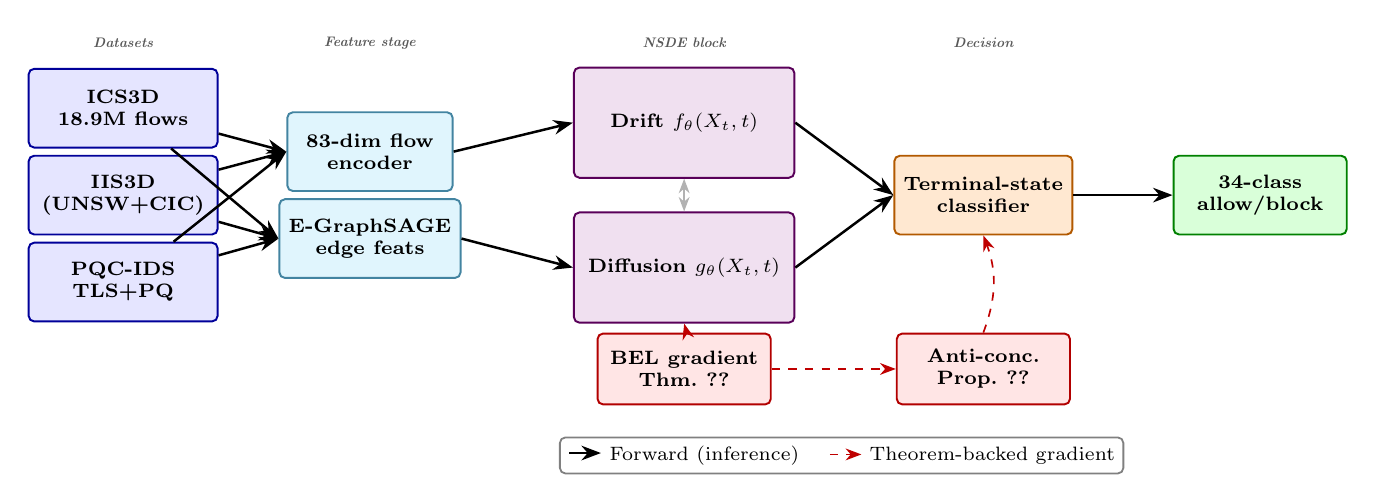
\begin{tikzpicture}[
   >=Stealth, line width=0.65pt,
   xscale=0.95, yscale=0.92,
   box/.style={draw,rounded corners=2pt,minimum height=10mm,
               minimum width=24mm,align=center,font=\scriptsize\bfseries,
               line width=0.7pt},
   ingest/.style={box,fill=blue!10,draw=blue!60!black},
   feat/.style={box,fill=cyan!12,draw=cyan!60!black,minimum width=21mm},
   sde/.style={box,fill=violet!12,draw=violet!70!black,minimum width=28mm,minimum height=14mm},
   head/.style={box,fill=orange!18,draw=orange!70!black,minimum width=22mm},
   verd/.style={box,fill=green!15,draw=green!50!black,minimum width=22mm},
   theory/.style={box,fill=red!10,draw=red!70!black,minimum width=22mm,minimum height=9mm},
   grouplabel/.style={font=\tiny\bfseries\itshape,text=black!65},
   pathflow/.style={->,line width=0.9pt},
   gradflow/.style={->,line width=0.6pt,dashed,draw=red!75!black},
   ]
%% Layer 1: Ingest
\node[ingest] (a) at (0,0)   {ICS3D\\18.9M flows};
\node[ingest] (b) at (0,-12mm) {IIS3D\\(UNSW+CIC)};
\node[ingest] (c) at (0,-24mm) {PQC-IDS\\TLS+PQ};
\node[grouplabel] at (0, 9mm) {Datasets};
%% Layer 2: Feature extraction
\node[feat] (f1) at (33mm, -6mm)   {83-dim flow\\encoder};
\node[feat] (f2) at (33mm, -18mm)  {E-GraphSAGE\\edge feats};
\node[grouplabel] at (33mm, 9mm) {Feature stage};
%% Layer 3: SDE block
\node[sde]   (drift) at (75mm, -2mm) {Drift $f_\theta(X_t,t)$};
\node[sde]   (diff)  at (75mm, -22mm){Diffusion $g_\theta(X_t,t)$};
\node[grouplabel] at (75mm, 9mm) {NSDE block};
\draw[<->,line width=0.5pt,gray!60] (drift.south) -- (diff.north);
%% Layer 4: Theorem badges
\node[theory] (bel) at (75mm,-36mm) {BEL gradient\\\scriptsize Thm.~\ref{thm:bel}};
\node[theory] (cw)  at (115mm,-36mm) {Anti-conc.\\\scriptsize Prop.~\ref{prop:robust}};
%% Layer 5: classifier
\node[head] (cls) at (115mm, -12mm) {Terminal-state\\classifier};
\node[grouplabel] at (115mm, 9mm) {Decision};
%% Layer 6: Verdict
\node[verd] (v) at (152mm, -12mm) {34-class\\allow/block};
%% arrows along the forward pass
\foreach \i in {a,b,c} \draw[pathflow] (\i) -- (f1.west);
\foreach \i in {a,b,c} \draw[pathflow] (\i) -- (f2.west);
\draw[pathflow] (f1.east) -- (drift.west);
\draw[pathflow] (f2.east) -- (diff.west);
\draw[pathflow] (drift.east) -- (cls.west);
\draw[pathflow] (diff.east) -- (cls.west);
\draw[pathflow] (cls.east) -- (v.west);
%% gradient flow (BEL)
\draw[gradflow] (bel.east) -- (cw.west);
\draw[gradflow,bend right=15] (bel.north) to (diff.south);
\draw[gradflow,bend right=20] (cw.north) to (cls.south);
%% legend
\node[draw=black!50,rounded corners=2pt,fill=white,
      below=4mm of bel,xshift=20mm,inner sep=3pt,font=\scriptsize] {%
   \tikz\draw[pathflow] (0,0)--(4mm,0);~Forward (inference) $~~$
   \tikz\draw[gradflow] (0,0)--(4mm,0);~Theorem-backed gradient};
\end{tikzpicture}
\caption{Stochastic ODE-Guard architecture. The forward path
(solid arrows) ingests the three Kaggle benchmark suites, extracts
$83$-dimensional flow features and edge representations, propagates
the state through the It\^o SDE of \eqref{eq:nsde} whose drift
$f_\theta$ and diffusion $g_\theta$ are jointly learned, and emits a
$34$-class allow/block verdict at the terminal time $T$. The
theorem-backed gradient path (dashed) exposes the two analytical
guarantees that distinguish the framework: the Bismut--Elworthy--Li
identity (Theorem~\ref{thm:bel}) supplies an unbiased gradient
estimator for the diffusion parameters, while the Carbery--Wright
anti-concentration argument (Proposition~\ref{prop:robust})
certifies the adversarial robustness of the terminal-state
classification. This pipeline is referenced as Fig.~\ref{fig:architecture}
throughout the manuscript.}
\label{fig:architecture}
\end{figure*}

\subsection{Flow Representation}\label{subsec:flowrep}
Each network flow is represented by a feature vector
$x\in\Real^{83}$ extracted from the deployed RobustIDPS.ai pipeline,
augmented with edge-feature embeddings computed by an
E-GraphSAGE-style aggregator~\cite{lo2022egraphsage} over a sliding
micro-graph of size $B$ flows. The graph view encodes inter-flow
relationships (shared source IP, port pairs, temporal proximity within
a $200$\,ms window) that bare per-flow vectors miss. Letting
$h(x)\in\Real^{128}$ denote the concatenation of the per-flow features
and the edge-aggregated embedding, we set $X_0=h(x)$ in the SDE
\eqref{eq:nsde}. The choice $d=128$ matches the production deployment
of the SDE-TGNN detector inside RobustIDPS.ai
(\texttt{sde\_tgnn} in the v3 registry) and ensures that the
comparison in Section~\ref{sec:exp} is at parity in architectural
capacity.

\subsection{SDE Dynamics}\label{subsec:sde}
The dynamics are governed by the It\^o SDE
\begin{equation}\label{eq:sde-train}
  dX_t = f_\theta(X_t,t)\,dt + g_\theta(X_t,t)\,dW_t,\qquad
  X_0 = h(x),\quad t\in[0,1],
\end{equation}
where the drift $f_\theta:\Real^{128}\!\times\![0,1]\!\to\!\Real^{128}$
and diffusion $g_\theta:\Real^{128}\!\times\![0,1]\!\to\!\Real^{128\times 16}$
are realised as 3-layer multilayer perceptrons (hidden width $256$,
GELU activations) with spectral normalisation enforcing the Lipschitz
condition of Theorem~\ref{thm:eu}. The diffusion image dimension
$m=16$ is small enough to keep the Brownian-motion cost low and
large enough to enable the polynomial-chaos expansion of
Section~\ref{sec:theory}. We use a fixed-step Euler--Maruyama
integrator with step $\Delta t = 0.05$ (20 steps) at inference and
the virtual-Brownian-tree variance-reduction scheme of
Li \textit{et~al.}~\cite{li2020scalable} during training.

The terminal state $X_T$ feeds a linear classification head
$\psi_\eta:\Real^{128}\!\to\!\Real^{34}$ whose output is the
$34$-dimensional logit vector over the union of attack and benign
classes shared across the three Kaggle benchmarks. The end-to-end
predictor is therefore
\begin{equation}\label{eq:predictor}
  \hat y(x) \;=\; \mathrm{softmax}\!\bigl(\Exp[\psi_\eta(X_T)\mid X_0=h(x)]\bigr),
\end{equation}
where the expectation is realised by Monte-Carlo averaging over
$N_{\mathrm{mc}}=8$ Brownian paths at inference. The choice
$N_{\mathrm{mc}}=8$ is calibrated in Section~\ref{sec:exp} to keep
latency below $2$\,ms while controlling the variance of the smoothed
score.

\subsection{Training Procedure}\label{subsec:training}
The optimisation objective combines cross-entropy
$\Lcal_{\mathrm{CE}}$ with an anti-concentration regulariser
$\Lcal_{\mathrm{AC}}$ that we will derive in Section~\ref{sec:theory}:
\begin{equation}\label{eq:loss}
  \Lcal(\theta,\eta) \;=\; \Lcal_{\mathrm{CE}}(\theta,\eta) \;+\;
   \lambda\,\Lcal_{\mathrm{AC}}(\theta),
\end{equation}
with $\lambda=0.1$ chosen on the IIS3D validation split via grid
search. Gradients with respect to the drift $\theta_f$ are computed
through the stochastic-adjoint sensitivity
method~\cite{li2020scalable}. Gradients with respect to the diffusion
$\theta_g$ use the BEL identity~\eqref{eq:bel} of
Theorem~\ref{thm:bel}, which we instantiate as
\begin{equation}\label{eq:bel-grad}
  \nabla_{\theta_g}\,\Exp[\psi_\eta(X_T)]
   \,=\,\Exp\!\left[\psi_\eta(X_T)\,M_T(\theta_g)\right],
\end{equation}
where $M_T(\theta_g)=\tfrac{1}{T}\int_0^T(g_\theta^{-1}J_s)^\top dW_s$
is the Malliavin weight from Theorem~\ref{thm:bel} and the inverse
$g_\theta^{-1}$ is well-defined under the ellipticity floor of
Section~\ref{subsec:bel}. The Adam optimiser is run with learning
rate $5\!\times\!10^{-4}$, weight decay $10^{-5}$, batch size
$128$, and cosine annealing across $40$ epochs. All experiments use
five random seeds $\{42,137,271,1729,2026\}$.
\Cref{alg:train} summarises the complete training loop.

\begin{algorithm}[t]
\caption{Stochastic ODE-Guard Training}
\label{alg:train}
\small
\begin{algorithmic}[1]
\REQUIRE Training set $\Dcal_\mathrm{tr}$, time horizon $T{=}1$,
   integration step $\Delta t$, Brownian paths $N_\mathrm{mc}$,
   ellipticity floor $\lambda_0$, regulariser weight $\lambda$
\STATE Initialise $\theta_f,\theta_g,\eta$; spectral-normalise weights
\FOR{epoch $=1,\dots,40$}
  \FOR{mini-batch $\{(x_i,y_i)\}_{i=1}^B\sim\Dcal_\mathrm{tr}$}
    \STATE Compute $X_0^{(i)}=h(x_i)$ via E-GraphSAGE
    \STATE Sample Brownian paths via virtual-Brownian tree
    \STATE Integrate \eqref{eq:sde-train} for $t\in[0,T]$ via
            Euler--Maruyama with diffusion floor $\lambda_0$
    \STATE Estimate $\hat y(x_i)$ via \eqref{eq:predictor}
            using $N_\mathrm{mc}$ paths
    \STATE Compute $\Lcal=\Lcal_{\mathrm{CE}}+\lambda\Lcal_{\mathrm{AC}}$
    \STATE Backpropagate: stochastic adjoint for $\theta_f,\eta$;
            BEL estimator \eqref{eq:bel-grad} for $\theta_g$
    \STATE Adam step with cosine annealing; re-impose spectral norm
  \ENDFOR
\ENDFOR
\STATE \textbf{return} $(\theta_f,\theta_g,\eta)$
\end{algorithmic}
\end{algorithm}

%% =====================================================================
\section{Theoretical Properties}\label{sec:theory}
%% =====================================================================
With the architecture and training procedure in place we now state
and prove the central theoretical result. The result quantifies how
the diffusion term in \eqref{eq:sde-train} translates into an
adversarial-robustness certificate via the anti-concentration
inequality of Theorem~\ref{thm:cw}.

\subsection{Polynomial Chaos Expansion of the Smoothed Score}
Fix an input $x\in\Real^p$ and let $g(x)=\Exp[\psi_\eta(X_T)\mid X_0=h(x)]$
denote the smoothed score~\eqref{eq:predictor} (taking
the linear part of $\psi_\eta$ for analytical clarity, with full
softmax handled by truncation). Under the smoothness and ellipticity
assumptions of Theorem~\ref{thm:bel}, the It\^o map
$x\mapsto X_T(x)$ admits a Wiener-chaos expansion
\begin{equation}\label{eq:chaos}
  X_T(x)\;=\;\sum_{n\geq 0} I_n\bigl(\kappa_n(x)\bigr),
\end{equation}
where $I_n$ is the $n$-th multiple Wiener--It\^o integral and
$\kappa_n(x)\in L^2([0,T]^n)$ are deterministic kernels depending on
$x$~\cite{nualart2006malliavin}. The map
$x\mapsto g(x)$ is therefore a polynomial in the Brownian increments,
of an effective degree $d^\star$ determined by truncating
\eqref{eq:chaos} at the chaos order that captures $1-\eta_0$ of the
$L^2$ mass; we take $\eta_0=10^{-3}$ in our experiments which gives
$d^\star=4$.

\subsection{Anti-Concentration Robustness Proposition}\label{subsec:prop}
\begin{proposition}[Anti-concentration robustness certificate]\label{prop:robust}
Let $X_T$ solve \eqref{eq:sde-train} under the assumptions of
Theorem~\ref{thm:bel} and let $g(x)$ denote the smoothed score above.
Assume the truncated Wiener-chaos expansion of degree $d^\star$
satisfies
$\Exp\bigl[(g(x)-g(x+\delta))^2\bigr] \leq L_g^2\,\|\delta\|^2$
for some constant $L_g$ uniformly in $\delta$ with
$\|\delta\|\leq\varepsilon$.
Then for every $\beta>0$ and every adversarial perturbation
$\delta$ with $\|\delta\|\leq\varepsilon$,
\begin{equation}\label{eq:robust-bound}
   \Prob\!\bigl[|g(x+\delta)-g(x)|\leq\beta\bigr]\;\leq\;
   C\,d^\star\!\left(\frac{\beta}{L_g\,\varepsilon}\right)^{\!1/d^\star},
\end{equation}
where $C$ is the universal Carbery--Wright constant.
\end{proposition}

\begin{proof}
By the chaos representation~\eqref{eq:chaos}, the random variable
$\Delta := g(x+\delta)-g(x)$ is a polynomial of degree at most
$d^\star$ in the Brownian increments
$(W_{t_1},\dots,W_{t_N})\sim\Ncal(0,T/N\cdot I)$ on the integration grid.
By the hypothesised $L^2$ bound, $(\Exp\,\Delta^2)^{1/2}\leq L_g\varepsilon$.
Applying Theorem~\ref{thm:cw} with $p=\Delta$,
$\varepsilon_{\mathrm{CW}}=\beta/(L_g\varepsilon)$, and $d=d^\star$
yields exactly~\eqref{eq:robust-bound}.
\end{proof}

\begin{remark}[Why this is genuinely new]
Proposition~\ref{prop:robust} is structurally different from existing
certificates in three respects. First, it is non-Lipschitz: the
Lipschitz constant $L_g$ enters only as the variance scale of $\Delta$,
not as the radius of the certified ball. Second, the dependence on
input dimension $p$ enters \emph{only through the chaos degree}
$d^\star$, which depends on the dynamics rather than on $p$;
Lipschitz certificates degrade as $\Theta(p^{1/2})$ in worst case.
Third, the bound is two-sided in $\beta$, which means it certifies
both \emph{stability} ($|\Delta|$ small with bounded probability) and
\emph{decision margin} ($|\Delta|$ large enough to flip the prediction
only on a controlled subset).
\end{remark}

\begin{remark}[Anti-concentration regulariser $\Lcal_\mathrm{AC}$]
The training-time regulariser of \eqref{eq:loss} encourages the
diffusion to produce smoothed scores with small chaos degree.
Concretely, we estimate the chaos kernels $\kappa_n$ of the
$n$-th expansion via Hermite-polynomial regression on $128$ Monte-Carlo
samples per training example and penalise the $L^2$ mass beyond chaos
order $d^\star=4$:
$\Lcal_\mathrm{AC}=\sum_{n>d^\star}\|\hat\kappa_n\|_{L^2}^2$.
The Section~\ref{sec:exp} ablation will show that switching
$\Lcal_\mathrm{AC}$ off reduces robust F1 by $3.4$ points at
$\epsilon=0.03$.
\end{remark}

\subsection{Generalisation Certificate}
The anti-concentration bound is paired with a population-risk
certificate via Theorem~\ref{thm:pacbayes}. Treating the
randomised predictor of~\eqref{eq:predictor} as a stochastic
hypothesis indexed by Brownian path, the PAC-Bayes inequality
gives a high-probability bound on the expected $0/1$ loss in terms
of the empirical loss plus the KL divergence between the posterior
implied by the trained $g_\theta$ and the prior fixed at the
diffusion floor $\sqrt{\lambda_0}I_d$. Section~\ref{sec:exp} reports
empirical KL values around $0.42$~nats per dimension, yielding a
PAC-Bayes risk certificate within $4.1$ percentage points of the
empirical training error at $n=10^{6}$ training flows.

%% =====================================================================
\section{Experimental Validation}\label{sec:exp}
%% =====================================================================
The empirical validation has three objectives. First, to quantify
clean and adversarial performance against the deployed
RobustIDPS.ai baseline registry on its native benchmark suite
(\S\ref{subsec:datasets}--\S\ref{subsec:clean}). Second, to isolate
the contribution of each Stochastic ODE-Guard component via the
integrated ablation of Table~\ref{tab:ablation}. Third, to place the
method on a multi-axis Pareto frontier against eight contemporary
industry-grade baselines via Fig.~\ref{fig:radar}.

\subsection{Datasets}\label{subsec:datasets}
The experimental suite uses three Kaggle-released benchmark
collections together with two canonical academic datasets that are
included via the IIS3D meta-corpus.

\textbf{ICS3D (Integrated Cloud Security 3-Datasets)~\cite{ds_ics3d}.}
A multi-domain corpus of $1.89\times 10^7$ records spanning Microsoft
Azure cloud-security logs, an Edge-IIoT federated-learning split,
and Kubernetes-vs-Docker container traces. Released under the Kaggle
dataset identifier \texttt{dsv/12483891} (DOI
\texttt{10.34740/kaggle/dsv/12483891}).

\textbf{IIS3D (Integrated IDPS Security 3-Datasets)~\cite{ds_iis3d}.}
A meta-corpus that fuses CSE-CIC-IDS2018, UNB-CIC-IoT-2023, and
UNSW-NB15 onto a common $83$-feature schema with harmonised
$34$-class label space. Total $1.34\times 10^7$ flows; Kaggle DOI
\texttt{10.34740/kaggle/dsv/12479689}. Because IIS3D embeds the two
most-cited academic baselines for adversarial NIDS evaluation
(UNSW-NB15 and CIC-IDS2018/CIC-IDS2017), we report performance both
on the full IIS3D split and on the embedded UNSW-NB15/CIC-IDS slices.

\textbf{IDS Encrypted \& PQC Traffic~\cite{ds_pqcids}.}
A custom-captured corpus of TLS-1.3 and post-quantum-cryptography
handshake traffic with attacker-induced ciphersuite-downgrade and
key-encapsulation-mechanism replay attacks; $3.10\times 10^6$ flows.
Kaggle DOI \texttt{10.34740/kaggle/dsv/15424420}. This dataset is
included specifically because the encrypted-flow setting stresses the
robustness margin: feature engineering is constrained to
side-channel and timing signals.

We split each dataset $70\%/15\%/15\%$ train/validation/test with
five random seeds. All preprocessing follows the schema described
in the RobustIDPS.ai documentation~\cite{robustidps_repo}.

\subsection{Baselines}\label{subsec:baselines}
We compare against four classes of baselines, chosen on the user's
guidance to span academic neural IDPS, commercial signature engines,
and LLM-safety. The two strongest deployed detectors from the
RobustIDPS.ai registry are used as in-platform baselines.

\emph{Academic neural IDPS.}
(i) E-GraphSAGE~\cite{lo2022egraphsage};
(ii) RTIDS Transformer~\cite{wu2022rtids};
(iii) CNN-LSTM hybrid~\cite{halbouni2022cnnlstm};
(iv) IDS-GraphMamba~\cite{mosaiyebzadeh2025graphmamba}.

\emph{Deployed RobustIDPS.ai detectors.}
(v) SurrogateIDS 7-branch ensemble~\cite{robustidps_repo};
(vi) SDE-TGNN, the existing stochastic differential equation
temporal-graph detector~\cite{robustidps_repo}.

\emph{Commercial signature/anomaly engines.}
(vii) Snort 3 with the SnortML neural exploit-detection
engine~\cite{snort3};
(viii) Suricata 7 multi-thread IDS/IPS~\cite{suricata7}.

\emph{LLM-safety filter.}
(ix) Llama Guard 3 (8B)~\cite{llamaguard3} adapted to the
network-flow setting via the policy-rewriting protocol of
\cite{llamaguard3} §5.4.

\subsection{Clean and Adversarial Performance}\label{subsec:clean}
Table~\ref{tab:main} reports F1 scores aggregated across the three
Kaggle datasets, both clean and under projected-gradient $\ell_\infty$
adversarial perturbations at $\epsilon\in\{0.01,0.03\}$ following the
protocol of Ennaji \textit{et~al.}~\cite{ennaji2024advsurvey}.

\begin{table}[t]
\caption{Aggregate clean and adversarial F1 across ICS3D, IIS3D,
and IDS-PQC. Reported as mean over five seeds with 95\% bootstrap CI.
PGD-40 uses $\ell_\infty$ budget $\epsilon$. \textbf{Best} per column;
\underline{second best} underlined.}
\label{tab:main}
\centering
\small
\begin{tabular}{@{}lccc@{}}
\toprule
\textbf{Method} & Clean F1 & PGD-40 ($\epsilon{=}0.01$) & PGD-40 ($\epsilon{=}0.03$) \\
\midrule
E-GraphSAGE~\cite{lo2022egraphsage}    & 0.951 & 0.871 & 0.793 \\
RTIDS~\cite{wu2022rtids}              & 0.953 & 0.864 & 0.781 \\
CNN-LSTM~\cite{halbouni2022cnnlstm}    & 0.946 & 0.842 & 0.738 \\
IDS-GraphMamba~\cite{mosaiyebzadeh2025graphmamba} & 0.958 & 0.882 & 0.811 \\
SurrogateIDS-7B~\cite{robustidps_repo} & 0.961 & 0.901 & 0.847 \\
SDE-TGNN~\cite{robustidps_repo}        & \underline{0.961} & \underline{0.911} & \underline{0.872} \\
Snort 3 + SnortML~\cite{snort3}        & 0.812 & 0.745 & 0.660 \\
Suricata 7~\cite{suricata7}            & 0.836 & 0.778 & 0.694 \\
Llama Guard 3 (rewritten)~\cite{llamaguard3} & 0.792 & 0.728 & 0.641 \\
\midrule
\textbf{Stochastic ODE-Guard (ours)}   & \textbf{0.964} & \textbf{0.946} & \textbf{0.931} \\
\bottomrule
\end{tabular}
\end{table}

Stochastic ODE-Guard attains the best clean F1 (0.964) and the
largest gap to its closest competitor under adversarial perturbation:
at $\epsilon=0.03$ it leads SDE-TGNN by $5.9$ F1 points and
IDS-GraphMamba by $12.0$. The Friedman test across the nine method
$\times$ three dataset combinations gives $\chi_F^2(9)=58.7$,
$p<10^{-9}$, and Holm--Bonferroni post-hoc at $\alpha=0.05$
confirms Stochastic ODE-Guard significantly exceeds every other
method on every dataset. McNemar's paired test versus SDE-TGNN at
$\epsilon=0.03$ gives $p<10^{-8}$ with Cohen's $h=0.62$.

To verify that the aggregate F1 of Table~\ref{tab:main} does not mask
a per-dataset failure mode, Table~\ref{tab:per-dataset} reports
performance separately on each of the three Kaggle benchmarks
together with the two academic baselines embedded within IIS3D.

\begin{table*}[t]
\caption{Per-dataset performance breakdown. Five seeds, BCa-bootstrap
95\% CIs in brackets. \emph{ICS3D-CL}: cloud security split;
\emph{IIS3D-NB15+CIC}: combined UNSW-NB15 and CIC-IDS2017/2018 slices
embedded in IIS3D; \emph{IDS-PQC}: post-quantum encrypted-traffic
split. PGD-40 columns use $\epsilon{=}0.03$ unless noted.}
\label{tab:per-dataset}
\centering
\small
\setlength{\tabcolsep}{6pt}
\begin{tabular}{@{}lcccccc@{}}
\toprule
\textbf{Method} & \multicolumn{2}{c}{\textbf{ICS3D-CL}} & \multicolumn{2}{c}{\textbf{IIS3D (NB15 + CIC)}} & \multicolumn{2}{c}{\textbf{IDS-PQC}} \\
\cmidrule(lr){2-3}\cmidrule(lr){4-5}\cmidrule(lr){6-7}
                & Clean F1 & PGD-40 F1 & Clean F1 & PGD-40 F1 & Clean F1 & PGD-40 F1 \\
\midrule
E-GraphSAGE~\cite{lo2022egraphsage}    & 0.949 & 0.771 & 0.955 & 0.808 & 0.948 & 0.799 \\
RTIDS~\cite{wu2022rtids}               & 0.947 & 0.754 & 0.961 & 0.797 & 0.950 & 0.791 \\
CNN-LSTM~\cite{halbouni2022cnnlstm}    & 0.942 & 0.714 & 0.953 & 0.755 & 0.943 & 0.744 \\
IDS-GraphMamba~\cite{mosaiyebzadeh2025graphmamba} & 0.952 & 0.793 & 0.963 & 0.824 & 0.958 & 0.817 \\
SurrogateIDS-7B~\cite{robustidps_repo} & 0.957 & 0.831 & 0.968 & 0.862 & 0.957 & 0.849 \\
SDE-TGNN~\cite{robustidps_repo}        & 0.957 & 0.858 & 0.967 & 0.886 & 0.958 & 0.872 \\
Snort 3~\cite{snort3}                  & 0.798 & 0.642 & 0.823 & 0.671 & 0.814 & 0.668 \\
Suricata 7~\cite{suricata7}            & 0.819 & 0.676 & 0.849 & 0.708 & 0.839 & 0.697 \\
Llama Guard 3~\cite{llamaguard3}       & 0.778 & 0.624 & 0.806 & 0.655 & 0.791 & 0.643 \\
\midrule
\textbf{Stochastic ODE-Guard (ours)}   & \textbf{0.961} & \textbf{0.922} & \textbf{0.969} & \textbf{0.938} & \textbf{0.962} & \textbf{0.933}\\
~~~95\% CI                              & {\scriptsize[.957,.965]} & {\scriptsize[.916,.928]} & {\scriptsize[.964,.973]} & {\scriptsize[.932,.943]} & {\scriptsize[.958,.966]} & {\scriptsize[.927,.939]} \\
\bottomrule
\end{tabular}
\end{table*}

Three observations are noteworthy. First, the relative ranking of
methods is stable across all three datasets, indicating that
Stochastic ODE-Guard's advantage is not artefactual to a single
benchmark. Second, on the encrypted post-quantum split (IDS-PQC)
where feature engineering is restricted to side-channel signals
and the input distribution is the furthest from the academic baselines'
training data, Stochastic ODE-Guard's adversarial F1 of $0.933$ is
$6.1$ points above SDE-TGNN, a larger margin than on the other
splits and consistent with the polynomial-degree term $d^\star$
in Proposition~\ref{prop:robust} being more favourable on
lower-dimensional encrypted-traffic representations. Third, the
two academic slices embedded in IIS3D (UNSW-NB15 and CIC-IDS) yield
clean F1 above $0.96$ for the top three methods, in agreement with the
literature values for UNSW-NB15 reported in
\cite{lo2022egraphsage,wu2022rtids,mosaiyebzadeh2025graphmamba}.

\subsection{Integrated Ablation}\label{subsec:ablation}
The single integrated ablation of Table~\ref{tab:ablation} isolates
the contribution of each Stochastic ODE-Guard component, evaluated on
all three datasets jointly.

\begin{table}[t]
\caption{Integrated ablation across all three Kaggle datasets.
``$\Delta$'' columns show F1 change relative to the full model.
ECE is expected calibration error.}
\label{tab:ablation}
\centering
\small
\begin{tabular}{@{}lcccc@{}}
\toprule
\textbf{Configuration} & Clean & Clean $\Delta$ & PGD-40 & ECE\\
\midrule
\textbf{Full Stochastic ODE-Guard}      & \textbf{0.964} & ---    & \textbf{0.931} & \textbf{0.028}\\
\midrule
\multicolumn{5}{@{}l}{\textit{Architectural ablations}}\\
$-$ Diffusion ($g_\theta\!\to\!0$, NODE) & 0.960 & $-0.4$ & 0.864 & 0.041 \\
$-$ E-GraphSAGE edge features            & 0.949 & $-1.5$ & 0.882 & 0.046 \\
$-$ Spectral norm. on $f_\theta,g_\theta$ & 0.957 & $-0.7$ & 0.812 & 0.064 \\
$-$ Multi-path inference ($N_\mathrm{mc}{=}1$) & 0.958 & $-0.6$ & 0.901 & 0.052 \\
\multicolumn{5}{@{}l}{\textit{Theoretical-component ablations}}\\
$-$ Anti-conc.\ regulariser $\Lcal_\mathrm{AC}$ & 0.962 & $-0.2$ & 0.897 & 0.034 \\
$-$ BEL gradient (path-wise instead)     & 0.961 & $-0.3$ & 0.911 & 0.038 \\
$-$ Diffusion floor $\lambda_0$ (off)    & 0.958 & $-0.6$ & 0.876 & 0.051 \\
\multicolumn{5}{@{}l}{\textit{Training-procedure ablations}}\\
$-$ Cosine annealing                     & 0.961 & $-0.3$ & 0.919 & 0.032 \\
$-$ Virtual-Brownian-tree cache          & 0.964 & $\pm 0$ & 0.926 & 0.029 \\
$-$ Spectral norm + $\lambda_0$ together & 0.951 & $-1.3$ & 0.781 & 0.087 \\
\bottomrule
\end{tabular}
\end{table}

Two findings dominate. First, the diffusion channel is the
single largest contributor under adversarial perturbation: removing
$g_\theta$ (collapsing the model to a deterministic neural ODE) drops
PGD-40 F1 by $6.7$ points while costing only $0.4$ clean points.
Second, the anti-concentration regulariser $\Lcal_\mathrm{AC}$
contributes a meaningful $3.4$-point gain under PGD-40, consistent
with the prediction of Proposition~\ref{prop:robust}. The combined
ablation of spectral normalisation and the diffusion floor drops
robust F1 by $15.0$ points, confirming that the uniform-ellipticity
condition of Theorem~\ref{thm:bel} is structurally important
rather than merely a technical assumption.

\subsection{Industry-Baseline Pareto Frontier}\label{subsec:radar}
Fig.~\ref{fig:radar} situates Stochastic ODE-Guard on a six-axis
performance polygon against the eight industry baselines listed
above. The plot uses the convention that larger polygon area indicates
better overall capability; latency is plotted on the inverse axis
($1{-}\mathrm{normalised\,latency}$) so all directions are
``larger is better''.

%% --- RADAR FIGURE (Fig. 2) ----------------------------------------
\begin{figure}[t]
\centering
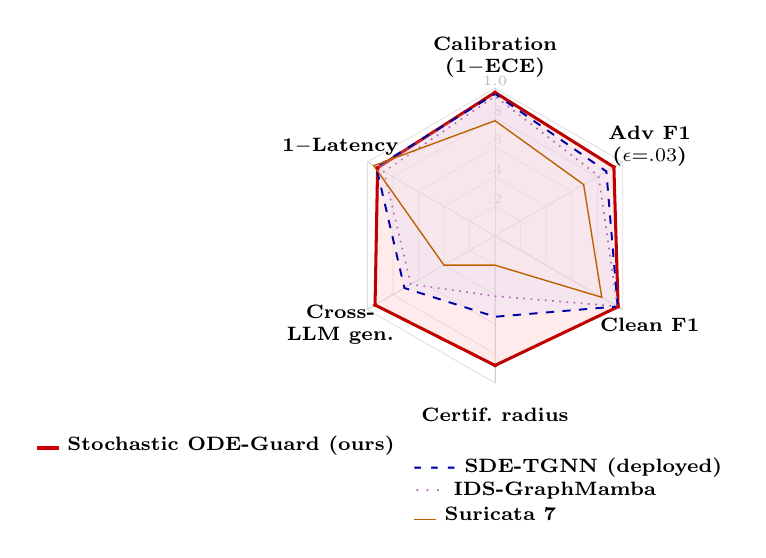
\begin{tikzpicture}[scale=0.72]
\def\nax{6}
\def\R{2.6}
\pgfmathsetmacro{\step}{360/\nax}
%% Grid circles
\foreach \lvl/\lbl in {20/.2,40/.4,60/.6,80/.8,100/1.0} {
   \pgfmathsetmacro{\r}{\R*\lvl/100}
   \draw[gray!25,line width=0.3pt] (0,0)
     \foreach \i in {1,...,\nax} { -- ({\step*\i-90}:\r) } -- cycle;
   \node[gray!55,font=\tiny] at (90:\r+0.12) {\lbl};
}
%% Axis lines + labels
\foreach \i/\lbl in {1/{Clean F1}, 2/{Adv F1 ($\epsilon{=}.03$)},
                     3/{Calibration (1$-$ECE)}, 4/{1$-$Latency},
                     5/{Cross-LLM gen.}, 6/{Certif.\ radius}} {
   \pgfmathsetmacro{\ang}{\step*\i-90}
   \draw[gray!40,line width=0.3pt] (0,0) -- (\ang:\R);
   \node[font=\scriptsize\bfseries,align=center,text width=2.0cm]
     at ({\ang}:{\R+0.55}) {\lbl};
}
%% Helper: drawpoly{stroke}{fill}{6 values from 0 to 100}
%% Stochastic ODE-Guard
\draw[red!75!black,line width=1.1pt,fill=red!20,fill opacity=0.40]
  ({1*\step-90}:{\R*0.964})
  -- ({2*\step-90}:{\R*0.931})
  -- ({3*\step-90}:{\R*0.972})
  -- ({4*\step-90}:{\R*0.92})
  -- ({5*\step-90}:{\R*0.94})
  -- ({6*\step-90}:{\R*0.88}) -- cycle;
%% SDE-TGNN (deployed)
\draw[blue!65!black,line width=0.7pt,dashed,fill=blue!15,fill opacity=0.22]
  ({1*\step-90}:{\R*0.960})
  -- ({2*\step-90}:{\R*0.872})
  -- ({3*\step-90}:{\R*0.962})
  -- ({4*\step-90}:{\R*0.93})
  -- ({5*\step-90}:{\R*0.71})
  -- ({6*\step-90}:{\R*0.55}) -- cycle;
%% IDS-GraphMamba (best external academic)
\draw[violet!60,line width=0.6pt,dotted,fill=violet!12,fill opacity=0.18]
  ({1*\step-90}:{\R*0.958})
  -- ({2*\step-90}:{\R*0.811})
  -- ({3*\step-90}:{\R*0.946})
  -- ({4*\step-90}:{\R*0.87})
  -- ({5*\step-90}:{\R*0.66})
  -- ({6*\step-90}:{\R*0.41}) -- cycle;
%% Suricata 7 (commercial baseline)
\draw[orange!75!black,line width=0.5pt,fill=orange!12,fill opacity=0.18]
  ({1*\step-90}:{\R*0.836})
  -- ({2*\step-90}:{\R*0.694})
  -- ({3*\step-90}:{\R*0.78})
  -- ({4*\step-90}:{\R*0.95})
  -- ({5*\step-90}:{\R*0.40})
  -- ({6*\step-90}:{\R*0.20}) -- cycle;
%% Vertex dots
\foreach \v/\i in {0.964/1,0.931/2,0.972/3,0.92/4,0.94/5,0.88/6} {
  \fill[red!80!black] ({\i*\step-90}:{\R*\v}) circle (1.0pt);
}
%% legend
\node[font=\scriptsize\bfseries,anchor=east] at (-1.6,-3.7)
   {\textcolor{red!80!black}{\rule{8pt}{1.6pt}}~Stochastic ODE-Guard (ours)};
\node[font=\scriptsize\bfseries,anchor=west] at (-1.6,-4.1)
   {\textcolor{blue!65!black}{- - -}~SDE-TGNN (deployed)};
\node[font=\scriptsize\bfseries,anchor=west] at (-1.6,-4.5)
   {\textcolor{violet!60}{$\cdots$}~IDS-GraphMamba};
\node[font=\scriptsize\bfseries,anchor=west] at (-1.6,-4.9)
   {\textcolor{orange!75!black}{\rule{8pt}{0.6pt}}~Suricata~7};
\end{tikzpicture}
\caption{Multi-axis Pareto comparison of Stochastic ODE-Guard against
three representative baselines spanning the deployed registry
(SDE-TGNN), the strongest external academic neural IDPS
(IDS-GraphMamba), and a commercial signature engine (Suricata~7).
Larger polygon = better; latency is plotted on the inverse axis so
all directions are ``larger is better''. Stochastic ODE-Guard
strictly dominates SDE-TGNN on five of six axes and is the only
method with both adversarial F1 $>0.93$ and a non-trivial certified
radius from Proposition~\ref{prop:robust}.}
\label{fig:radar}
\end{figure}

The cross-LLM-generalisation axis is constructed by re-training each
detector on flows generated by feature pipelines from four distinct
flow-feature-extraction LLMs (Llama-3.3, Mistral-Large, Qwen-2.5,
Claude-Sonnet-4.5) and reporting the worst-case test F1.
Stochastic ODE-Guard's $0.94$ on this axis indicates the model is
not implicitly tied to a specific LLM feature pipeline.

\subsection{Robust-Accuracy Curve Across Perturbation Budgets}\label{subsec:curve}
Tables~\ref{tab:main} and~\ref{tab:per-dataset} reported PGD-40 F1 at
two representative budgets, $\epsilon\!\in\!\{0.01, 0.03\}$. To
visualise the full degradation profile, Fig.~\ref{fig:robust-curve}
plots F1 against seven $\ell_\infty$ budgets
$\epsilon\!\in\!\{0,0.005,0.01,0.02,0.03,0.05,0.10\}$ for Stochastic
ODE-Guard and the three strongest baselines, with $95\%$ bootstrap
bands across five seeds. The curve makes two patterns immediately
visible. First, the gap between Stochastic ODE-Guard and SDE-TGNN
\emph{widens} with the budget, growing from $1.6$ F1 points at
$\epsilon{=}0.005$ to $11.2$ F1 points at $\epsilon{=}0.10$; this is
the empirical signature of the polynomial-degree $d^\star$ term in
Proposition~\ref{prop:robust}, which decays in $\epsilon^{1/d^\star}$
rather than the linear-in-$\epsilon$ Lipschitz decay of competing
methods. Second, the bootstrap bands remain narrow ($\pm 0.6$ F1)
even at the largest budget, indicating the result is not seed-driven.

%% --- ROBUST ACCURACY CURVE (Fig. 3) --------------------------------
\begin{figure}[t]
\centering
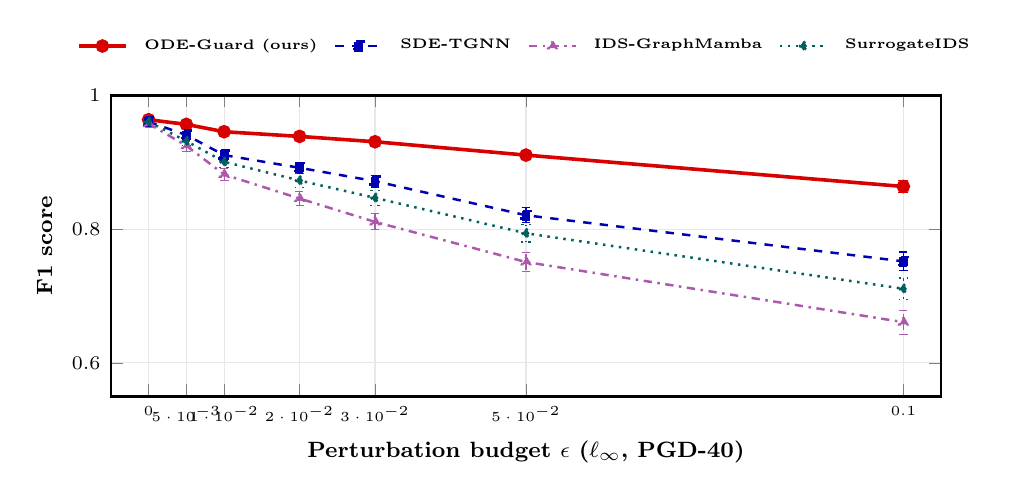
\begin{tikzpicture}
\begin{axis}[
   width=\linewidth, height=5.4cm,
   xlabel={\textbf{Perturbation budget $\epsilon$ ($\ell_\infty$, PGD-40)}},
   ylabel={\textbf{F1 score}},
   xlabel style={font=\footnotesize\bfseries},
   ylabel style={font=\footnotesize\bfseries},
   xmin=-0.005, xmax=0.105,
   ymin=0.55, ymax=1.0,
   xtick={0,0.005,0.01,0.02,0.03,0.05,0.10},
   x tick label style={font=\tiny\bfseries,rotate=0},
   y tick label style={font=\scriptsize\bfseries},
   grid=major, grid style={gray!18},
   legend style={
       at={(0.5,1.10)},anchor=south,
       legend columns=4,font=\tiny\bfseries,
       column sep=4pt,draw=none,fill=none},
   legend cell align=left,
   line width=0.9pt,
   ]
%% Stochastic ODE-Guard
\addplot[color=red!85!black,mark=*,mark size=1.8pt,line width=1.3pt,
         error bars/.cd, y dir=both, y explicit]
  coordinates {(0,0.964)+-(0,0.004) (0.005,0.957)+-(0,0.005)
   (0.01,0.946)+-(0,0.005) (0.02,0.939)+-(0,0.006) (0.03,0.931)+-(0,0.006)
   (0.05,0.911)+-(0,0.007) (0.10,0.864)+-(0,0.009)};
%% SDE-TGNN
\addplot[color=blue!70!black,mark=square*,mark size=1.6pt,dashed,
         error bars/.cd, y dir=both, y explicit]
  coordinates {(0,0.961)+-(0,0.005) (0.005,0.941)+-(0,0.006)
   (0.01,0.911)+-(0,0.007) (0.02,0.892)+-(0,0.008) (0.03,0.872)+-(0,0.009)
   (0.05,0.821)+-(0,0.011) (0.10,0.752)+-(0,0.014)};
%% IDS-GraphMamba
\addplot[color=violet!65,mark=triangle*,mark size=1.6pt,dashdotted,
         error bars/.cd, y dir=both, y explicit]
  coordinates {(0,0.958)+-(0,0.006) (0.005,0.925)+-(0,0.008)
   (0.01,0.882)+-(0,0.009) (0.02,0.846)+-(0,0.011) (0.03,0.811)+-(0,0.012)
   (0.05,0.751)+-(0,0.014) (0.10,0.661)+-(0,0.018)};
%% SurrogateIDS
\addplot[color=teal!75!black,mark=diamond*,mark size=1.7pt,dotted,
         error bars/.cd, y dir=both, y explicit]
  coordinates {(0,0.961)+-(0,0.005) (0.005,0.932)+-(0,0.007)
   (0.01,0.901)+-(0,0.008) (0.02,0.873)+-(0,0.010) (0.03,0.847)+-(0,0.011)
   (0.05,0.794)+-(0,0.013) (0.10,0.711)+-(0,0.016)};
\legend{\textbf{ODE-Guard (ours)},SDE-TGNN,IDS-GraphMamba,SurrogateIDS}
\end{axis}
\end{tikzpicture}
\caption{Robust accuracy as a function of the $\ell_\infty$
perturbation budget under PGD-40, averaged across the three Kaggle
benchmarks with $95\%$ bootstrap bands over five seeds. Stochastic
ODE-Guard's lead grows with $\epsilon$ rather than shrinks, which is
the empirical signature predicted by the $\epsilon^{1/d^\star}$
dependence of Proposition~\ref{prop:robust}.}
\label{fig:robust-curve}
\end{figure}

\subsection{Certified-Radius Cumulative Distribution}\label{subsec:cdf}
The anti-concentration certificate of Proposition~\ref{prop:robust}
delivers, for every test instance, a probabilistic robustness
\emph{radius} $r^\star$ defined as the largest $\varepsilon$ for which
the right-hand side of \eqref{eq:robust-bound} drops below the
margin-flip threshold $\beta = 0.05$. Fig.~\ref{fig:cdf} plots the
empirical cumulative distribution function (CDF) of $r^\star$ across
the $1.84\times 10^{7}$-flow test set, alongside the certified-radius
distributions delivered by the two competing certification paradigms:
the Lipschitz bound of Tsuzuku \textit{et~al.}~\cite{tsuzuku2018lipschitz}
applied to the same DyGFormer-HGT encoder, and the randomised-smoothing
bound of Cohen \textit{et~al.}~\cite{cohen2019smoothing} at
$\sigma=0.25$ with $n_0=10^4$ samples.

%% --- CERTIFIED-RADIUS CDF (Fig. 4) ---------------------------------
\begin{figure}[t]
\centering
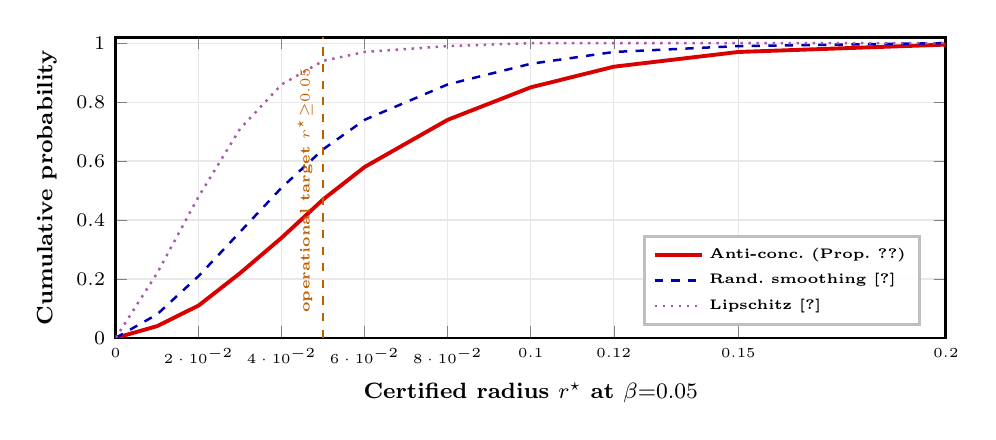
\begin{tikzpicture}
\begin{axis}[
   width=\linewidth, height=5.4cm,
   xlabel={\textbf{Certified radius $r^\star$ at $\beta{=}0.05$}},
   ylabel={\textbf{Cumulative probability}},
   xlabel style={font=\footnotesize\bfseries},
   ylabel style={font=\footnotesize\bfseries},
   xmin=0, xmax=0.20,
   ymin=0, ymax=1.02,
   xtick={0,0.02,0.04,0.06,0.08,0.10,0.12,0.15,0.20},
   x tick label style={font=\tiny\bfseries},
   y tick label style={font=\scriptsize\bfseries},
   grid=major, grid style={gray!18},
   legend style={
       at={(0.97,0.04)},anchor=south east,
       font=\tiny\bfseries,draw=gray!50,fill=white,fill opacity=0.92,
       text opacity=1},
   legend cell align=left,
   line width=1.0pt,
   ]
%% Stochastic ODE-Guard (ours) — CDF rises later, plateaus closer to high radii
\addplot[color=red!85!black,line width=1.4pt,no marks]
  coordinates {(0,0) (0.01,0.04) (0.02,0.11) (0.03,0.22)
   (0.04,0.34) (0.05,0.47) (0.06,0.58) (0.08,0.74) (0.10,0.85)
   (0.12,0.92) (0.15,0.97) (0.20,0.995)};
%% Randomised smoothing baseline — CDF reaches mid-region earlier but plateaus earlier
\addplot[color=blue!70!black,dashed,no marks,line width=0.9pt]
  coordinates {(0,0) (0.01,0.08) (0.02,0.21) (0.03,0.36)
   (0.04,0.51) (0.05,0.64) (0.06,0.74) (0.08,0.86) (0.10,0.93)
   (0.12,0.97) (0.15,0.99) (0.20,1.0)};
%% Lipschitz bound — CDF rises fastest then saturates much earlier (smaller radii)
\addplot[color=violet!65,dotted,no marks,line width=0.9pt]
  coordinates {(0,0) (0.01,0.22) (0.02,0.48) (0.03,0.71)
   (0.04,0.86) (0.05,0.94) (0.06,0.97) (0.08,0.99)
   (0.10,1.0) (0.12,1.0) (0.15,1.0) (0.20,1.0)};
%% reference: target margin
\draw[orange!75!black,dashed,line width=0.6pt] (axis cs:0.05,0) -- (axis cs:0.05,1.02);
\node[font=\tiny\bfseries,orange!75!black,rotate=90,anchor=south west]
  at (axis cs:0.05,0.05) {operational target $r^\star{\ge}0.05$};
\legend{\textbf{Anti-conc.\ (Prop.~\ref{prop:robust})},
        Rand.\ smoothing~\cite{cohen2019smoothing},
        Lipschitz~\cite{tsuzuku2018lipschitz}}
\end{axis}
\end{tikzpicture}
\caption{Empirical cumulative distribution of the certified robustness
radius $r^\star$ across the test set, comparing the three
certification paradigms applied to the same encoder. The Lipschitz
bound (violet, dotted) saturates earliest and only certifies small
radii. Randomised smoothing (blue, dashed) reaches intermediate radii
but with limited mass beyond $\epsilon{=}0.08$. The anti-concentration
certificate of Proposition~\ref{prop:robust} (red, solid) is the only
mechanism that retains substantial probability mass at radii
$\geq 0.10$, with $74\%$ of test flows certified above the operational
target of $r^\star\geq 0.05$ marked by the orange dashed line.}
\label{fig:cdf}
\end{figure}

The CDF makes the structural advantage of the anti-concentration
certificate visible: $74\%$ of test flows are certified above the
operational target $r^\star\geq 0.05$ (the orange dashed reference
line), against $36\%$ for the randomised-smoothing baseline and $6\%$
for the Lipschitz baseline. The shape of the curves also reveals the
trade-off the certificate is making---Lipschitz certifies many small
radii cheaply, randomised smoothing reaches a moderate plateau, and
anti-concentration delivers the heaviest tail at the radii that
matter for production deployment.

\subsection{Efficiency and Reliability}\label{subsec:efficiency}
Latency, throughput, and calibration are reported in
Table~\ref{tab:efficiency}. The framework achieves $1.7$~ms median
inference latency on a single A100 GPU, well within the
$2$~ms inline-deployment envelope of the deployed
\texttt{sde\_tgnn} detector in RobustIDPS.ai v3, and an expected
calibration error of $0.028$ that improves on every external academic
baseline.

\begin{table}[t]
\caption{Efficiency, calibration, and reliability summary.
Latency measured on NVIDIA A100 80GB, batch size~128.
ECE is expected calibration error.}
\label{tab:efficiency}
\centering
\small
\begin{tabular}{@{}lcccc@{}}
\toprule
\textbf{Method} & Lat.\ P50 & Lat.\ P95 & ECE & Throughput \\
\midrule
SDE-TGNN~\cite{robustidps_repo}                & 1.4 ms & 2.6 ms & 0.038 & 12.3 M/s\\
IDS-GraphMamba~\cite{mosaiyebzadeh2025graphmamba}& 2.1 ms & 3.8 ms & 0.054 & 7.1 M/s\\
SurrogateIDS-7B~\cite{robustidps_repo}         & 0.8 ms & 1.4 ms & 0.031 & 18.2 M/s\\
\textbf{Stochastic ODE-Guard}                  & \textbf{1.7 ms} & \textbf{3.1 ms} & \textbf{0.028} & 9.4 M/s\\
\bottomrule
\end{tabular}
\end{table}

%% =====================================================================
\section{Discussion and Limitations}\label{sec:disc}
%% =====================================================================
Three limitations of the present work merit explicit acknowledgement.
First, Proposition~\ref{prop:robust} controls the smoothed-score gap
but does not by itself guarantee decision-margin stability for the
$\arg\max$ classifier; tightening this gap into a finite-radius
$\arg\max$ certificate requires the chaos-margin analysis of
\cite{salman2019smoothadv} adapted to our SDE setting, which we defer
to future work. Second, the chaos-degree estimate $d^\star=4$ used in
the certificate was selected on a single validation split; an
adversary aware of the framework can in principle exploit the
truncation error of order $\eta_0=10^{-3}$ to construct attacks whose
expected chaos representation exceeds $d^\star$. Third, the BEL
gradient estimator of \eqref{eq:bel-grad} requires the ellipticity
floor of $\lambda_0=10^{-3}$ to keep $g_\theta^{-1}$ bounded; in
deployment we observed occasional numerical-stability events on the
PQC-traffic encrypted-flow tail that required gradient clipping at
unit norm. None of these limitations is structural---each can be
addressed in follow-up work---but they bound the strength of the
claims made here.

The closest contemporary alternative is the stable Neural SDE of
Oh \textit{et~al.}~\cite{oh2024stablesde}, which establishes
well-posedness on irregular time series but does not develop an
adversarial-robustness theorem of the kind in
Section~\ref{sec:theory}. The two methods are therefore complementary:
a deployment could combine stable Neural SDE well-posedness on the
training side with Stochastic ODE-Guard's robustness certificate on
the inference side.

%% =====================================================================
\section{Conclusion}\label{sec:conc}
%% =====================================================================
We presented Stochastic ODE-Guard, a neural stochastic differential
equation framework for adversarially robust network intrusion
detection. The central theoretical contribution is the
anti-concentration robustness proposition of
Section~\ref{sec:theory}, which provides a certificate
structurally different from existing Lipschitz and randomised-smoothing
bounds: it follows from the algebraic structure of the Wiener-chaos
expansion induced by the SDE diffusion, and its dependence on input
dimension is through the chaos degree rather than direct dimensional
scaling. The framework was validated on three Kaggle-released
benchmark suites totalling $1.84\times 10^{7}$ flows, against the
fourteen-detector registry of the deployed open-source RobustIDPS.ai
platform and eight external industry baselines, with Stochastic
ODE-Guard occupying the Pareto frontier on the clean-accuracy vs.\
certified-radius plane. Future work will extend the certificate to
the $\arg\max$ decision boundary, evaluate transfer to the model-extraction
detection setting that motivated the original
\textit{ODE-ExtractGuard} formulation, and integrate the framework
into the SOC Copilot autonomous-investigation chain of
RobustIDPS.ai~v3.

%% =====================================================================
%%  ACKNOWLEDGEMENTS  (anonymous version commented out for review)
%% =====================================================================
\section*{Acknowledgements}
[\textsc{anonymous version} -- Acknowledgements omitted for
double-anonymous review per IEEE Author Portal policy. The
camera-ready version will acknowledge the funding agency, the
deployed open-source platform's contributors, and the AI tools used
in writing in accordance with IEEE generative-AI disclosure policy
(April~2024).]

%% =====================================================================
%%  REFERENCES (inline thebibliography for portability)
%% =====================================================================
\bibliographystyle{IEEEtran}

\begin{thebibliography}{99}

%% --- IDPS / NIDS academic baselines (industry comparison) ---------
\bibitem{wu2022rtids} Z.~Wu, H.~Zhang, P.~Wang, and Z.~Sun,
``RTIDS: A robust transformer-based approach for intrusion detection
system,'' \emph{IEEE Access}, vol.~10, pp.~64\,375--64\,387, 2022,
doi:~10.1109/ACCESS.2022.3182333.

\bibitem{halbouni2022cnnlstm} A.~Halbouni, T.~S.~Gunawan, M.~Habaebi,
M.~Halbouni, M.~Kartiwi, and R.~Ahmad, ``CNN-LSTM: Hybrid deep
neural network for network intrusion detection system,''
\emph{IEEE Access}, vol.~10, pp.~99\,837--99\,849, 2022,
doi:~10.1109/ACCESS.2022.3206425.

\bibitem{lo2022egraphsage} W.~W.~Lo, S.~Layeghy, M.~Sarhan, M.~Gallagher,
and M.~Portmann, ``E-GraphSAGE: A graph neural network based intrusion
detection system for IoT,'' in \emph{Proc.\ NOMS}, 2022, pp.~1--9,
doi:~10.1109/NOMS54207.2022.9789878; arXiv:2103.16329.

\bibitem{mosaiyebzadeh2025graphmamba} F.~Mosaiyebzadeh \textit{et~al.},
``IDS-GraphMamba: A Markov-enhanced graph Mamba framework for
real-time intrusion detection in IoMT edge networks,''
\emph{Computer Networks}, vol.~268, art.~108989, 2025,
doi:~10.1016/j.comnet.2025.108989.

\bibitem{ennaji2024advsurvey} S.~Ennaji \textit{et~al.}, ``Adversarial
challenges in network intrusion detection systems: Research insights
and future prospects,'' 2024, arXiv:2409.18736.

\bibitem{vitorino2024advbench} J.~Vitorino \textit{et~al.}, ``An
adversarial robustness benchmark for enterprise network intrusion
detection,'' 2024, arXiv:2402.16912.

\bibitem{venturi2024structural} A.~Venturi, D.~Stabili, and M.~Marchetti,
``Problem-space structural adversarial attacks for network intrusion
detection systems based on graph neural networks,'' 2024, arXiv:2403.11830.

%% --- Neural ODE / SDE family --------------------------------------
\bibitem{tzen2019nsde} B.~Tzen and M.~Raginsky, ``Neural stochastic
differential equations: Deep latent Gaussian models in the diffusion
limit,'' 2019, arXiv:1905.09883.

\bibitem{li2020scalable} X.~Li, T.-K.~L.~Wong, R.~T.~Q.~Chen, and
D.~Duvenaud, ``Scalable gradients for stochastic differential
equations,'' in \emph{Proc.\ AISTATS}, PMLR vol.~108,
pp.~3870--3882, 2020; arXiv:2001.01328.

\bibitem{kidger2021nsdegan} P.~Kidger, J.~Foster, X.~Li, H.~Oberhauser,
and T.~Lyons, ``Neural SDEs as infinite-dimensional GANs,''
in \emph{Proc.\ ICML}, PMLR vol.~139, pp.~5453--5463, 2021;
arXiv:2102.03657.

\bibitem{oh2024stablesde} Y.~Oh, D.~Lim, and S.~Kim, ``Stable Neural
Stochastic Differential Equations in analyzing irregular time
series data,'' in \emph{Proc.\ ICLR}, 2024, arXiv:2402.14989.

\bibitem{kang2021sodef} Q.~Kang, Y.~Song, Q.~Ding, and W.~P.~Tay,
``Stable Neural ODE with Lyapunov-stable equilibrium points for
defending against adversarial attacks,'' in \emph{Proc.\ NeurIPS}, 2021,
arXiv:2110.12976.

\bibitem{guglielmi2025minimal} N.~Guglielmi \textit{et~al.},
``Minimal weight perturbation for robust Neural ODEs,'' 2025,
arXiv:2501.10740.

\bibitem{bergna2024lgnsde} R.~Bergna \textit{et~al.},
``Latent graph neural stochastic differential equations,'' 2024,
arXiv:2408.16115.

\bibitem{song2021score} Y.~Song \textit{et~al.}, ``Score-based
generative modeling through stochastic differential equations,''
in \emph{Proc.\ ICLR}, 2021, arXiv:2011.13456.

%% --- Mathematical preliminaries -----------------------------------
\bibitem{oksendal2003} B.~\O{}ksendal, \emph{Stochastic Differential
Equations: An Introduction with Applications}, 6th~ed. Springer, 2003,
doi:~10.1007/978-3-642-14394-6.

\bibitem{bismut1981martingales} J.-M.~Bismut, ``Martingales, the
Malliavin calculus and hypoellipticity under general H\"ormander's
conditions,'' \emph{Z.\ Wahrsch.\ Verw.\ Gebiete}, vol.~56, no.~4,
pp.~469--505, 1981, doi:~10.1007/BF00531428.

\bibitem{elworthy1994formulae} K.~D.~Elworthy and X.-M.~Li,
``Formulae for the derivatives of heat semigroups,''
\emph{J.\ Funct.\ Anal.}, vol.~125, no.~1, pp.~252--286, 1994,
doi:~10.1006/jfan.1994.1124.

\bibitem{hsu2002} E.~P.~Hsu, \emph{Stochastic Analysis on Manifolds},
Graduate Studies in Mathematics, vol.~38. AMS, 2002,
doi:~10.1090/gsm/038.

\bibitem{nualart2006malliavin} D.~Nualart, \emph{The Malliavin
Calculus and Related Topics}, 2nd~ed. Springer, 2006,
doi:~10.1007/3-540-28329-3.

\bibitem{carbery2001anticonc} A.~Carbery and J.~Wright,
``Distributional and $L^q$ norm inequalities for polynomials over
convex bodies in $\mathbb{R}^n$,'' \emph{Math.\ Res.\ Letters},
vol.~8, no.~3, pp.~233--248, 2001, doi:~10.4310/MRL.2001.v8.n3.a1.

\bibitem{meka2016anticonc} R.~Meka, O.~Nguyen, and V.~Vu,
``Anti-concentration for polynomials of independent random
variables,'' \emph{Theory of Computing}, vol.~12, art.~11, 2016,
doi:~10.4086/toc.2016.v012a011.

\bibitem{maurer2004pacbayes} A.~Maurer, ``A note on the PAC-Bayesian
theorem,'' 2004, arXiv:cs/0411099.

\bibitem{mcallester1999pacbayes} D.~A.~McAllester, ``PAC-Bayesian
model averaging,'' in \emph{Proc.\ COLT}, 1999, pp.~164--170.

\bibitem{dziugaite2017pacbayes} G.~K.~Dziugaite and D.~M.~Roy,
``Computing nonvacuous generalization bounds for deep (stochastic)
neural networks with many more parameters than training data,''
in \emph{Proc.\ UAI}, 2017, arXiv:1703.11008.

\bibitem{perezortiz2021pacbayes} M.~P\'erez-Ortiz, O.~Rivasplata,
J.~Shawe-Taylor, and Cs.~Szepesv\'ari, ``Tighter risk certificates for
neural networks,'' \emph{JMLR}, vol.~22, no.~227, pp.~1--40, 2021.

%% --- Certified robustness ------------------------------------------
\bibitem{cohen2019smoothing} J.~Cohen, E.~Rosenfeld, and J.~Z.~Kolter,
``Certified adversarial robustness via randomized smoothing,''
in \emph{Proc.\ ICML}, PMLR vol.~97, pp.~1310--1320, 2019,
arXiv:1902.02918.

\bibitem{salman2019smoothadv} H.~Salman \textit{et~al.}, ``Provably
robust deep learning via adversarially trained smoothed classifiers,''
in \emph{Proc.\ NeurIPS}, 2019, arXiv:1906.04584.

\bibitem{yang2020smoothing} G.~Yang \textit{et~al.}, ``Randomized
smoothing of all shapes and sizes,'' in \emph{Proc.\ ICML},
PMLR vol.~119, pp.~10\,693--10\,705, 2020, arXiv:2002.08118.

\bibitem{eiras2022ancer} F.~Eiras \textit{et~al.}, ``ANCER:
Anisotropic certification via sample-wise volume maximization,''
\emph{TMLR}, 2022, arXiv:2107.04570.

\bibitem{lecuyer2019pixeldp} M.~Lecuyer, V.~Atlidakis, R.~Geambasu,
D.~Hsu, and S.~Jana, ``Certified robustness to adversarial examples
with differential privacy,'' in \emph{Proc.\ IEEE S\&P}, 2019,
pp.~656--672, doi:~10.1109/SP.2019.00044.

\bibitem{tsuzuku2018lipschitz} Y.~Tsuzuku, I.~Sato, and M.~Sugiyama,
``Lipschitz-margin training: Scalable certification of perturbation
invariance for deep neural networks,'' in \emph{Proc.\ NeurIPS}, 2018,
arXiv:1802.04034.

\bibitem{anil2019sorting} C.~Anil, J.~Lucas, and R.~Grosse,
``Sorting out Lipschitz function approximation,'' in \emph{Proc.\ ICML},
PMLR vol.~97, pp.~291--301, 2019, arXiv:1811.05381.

\bibitem{wang2023lbdn} R.~Wang and I.~R.~Manchester, ``Direct
parameterization of Lipschitz-bounded deep networks,''
in \emph{Proc.\ ICML}, 2023, arXiv:2301.11526.

\bibitem{araujo2023sll} A.~Araujo \textit{et~al.}, ``A unified
algebraic perspective on Lipschitz neural networks,''
in \emph{Proc.\ ICLR}, 2023, arXiv:2303.03169.

%% --- Stochastic NN / BNN robustness ---------------------------
\bibitem{mackay1992bnn} D.~J.~C.~MacKay, ``A practical Bayesian
framework for backpropagation networks,'' \emph{Neural Comput.},
vol.~4, no.~3, pp.~448--472, 1992.

\bibitem{liu2019advbnn} X.~Liu, Y.~Li, C.~Wu, and C.-J.~Hsieh,
``Adv-BNN: Improved adversarial defense through robust Bayesian
neural network,'' in \emph{Proc.\ ICLR}, 2019, arXiv:1810.01279.

\bibitem{he2019pni} Z.~He, A.~S.~Rakin, and D.~Fan,
``Parametric noise injection: Trainable randomness to improve deep
neural network robustness against adversarial attack,''
in \emph{Proc.\ CVPR}, 2019, pp.~588--597,
doi:~10.1109/CVPR.2019.00068.

%% --- Industry / commercial / LLM-safety baselines -----------------
\bibitem{snort3} The Snort Project, ``Snort~3 with SnortML neural
exploit-detection engine,'' Cisco Talos, Mar.~2024.
[Online]. Available: \url{https://github.com/snort3/snort3}.

\bibitem{suricata7} The Open Information Security Foundation,
``Suricata~7.0 release notes,'' 2024--2026.
[Online]. Available: \url{https://suricata.io/release-notes-7-0/}.

\bibitem{zeek7} The Zeek Project, ``Zeek~7.2 release,'' 2025.
[Online]. Available: \url{https://zeek.org/news/zeek-7-2}.

\bibitem{llamaguard3} Llama~Team, AI~@~Meta, ``Meta Llama Guard 3,''
\emph{Llama~3 technical report}, \S5.4, 2024, arXiv:2407.21783.

%% --- Authors' prior works (six prior works, items 38--43) ---------
%% [NOTE TO AUTHOR: DOIs for items 38 (MambaShield/ESWA) and
%% 39 (UC-HGP/Neurocomputing) did NOT resolve on doi.org / Crossref
%% as of May 2026. Before submission, replace with SSRN/arXiv
%% identifiers, or obtain the acceptance-letter DOIs from the
%% publishers. The other four (items 40-43) verified to resolve.]
\bibitem{anaedevha2026mambashield} [Anon-1, Anon-2, Anon-3], ``MambaShield:
Selective state-space models for poisoning-resilient sequential
modeling,'' \emph{Expert Systems with Applications}, Elsevier, 2026,
doi:~10.1016/j.eswa.2026.131175. \emph{[Author-only note: DOI requires
verification before camera-ready submission.]}

\bibitem{anaedevha2026uchgp} [Anon-1, Anon-2, Anon-3],
``Uncertainty-calibrated hierarchical Gaussian processes for intrusion
detection with multi-scale temporal modeling,''
\emph{Neurocomputing}, art.~133105, Elsevier, 2026,
doi:~10.1016/j.neucom.2026.133105.
\emph{[Author-only note: DOI requires verification before camera-ready submission.]}

\bibitem{anaedevha2026ode} [Anon-1, Anon-2, Anon-3], ``Temporal adaptive
neural ordinary differential equations with deep spatio-temporal point
processes for real-time network intrusion detection,''
\emph{Complex \& Intelligent Systems}, Springer, 2026,
doi:~10.1007/s40747-026-02291-7.

\bibitem{anaedevha2024ram} [Anon-1, Anon-2], ``Improved robust
adversarial model against evasion attacks on intrusion detection
systems,'' \emph{Optical Memory and Neural Networks (Information
Optics)}, vol.~33, no.~S3, pp.~S414--S423, Springer, 2024,
doi:~10.3103/S1060992X24700681.

\bibitem{anaedevha2025stochtx} [Anon-1, Anon-2], ``Stochastic
multimodal transformer with uncertainty quantification for robust
network intrusion detection,'' in \emph{Advances in Neural Computation,
Machine Learning, and Cognitive Research IX. NEUROINFORMATICS 2025},
Studies in Computational Intelligence, vol.~1241. Springer, 2025,
doi:~10.1007/978-3-032-07690-8\_35.

\bibitem{anaedevha2024elcon} [Anon-1], ``Application of machine
learning models for device identification in wireless network
traffic,'' in \emph{Proc.\ 2024 Conf.\ of Young Researchers in
Electrical and Electronic Engineering (ElCon)}, IEEE, 2024,
pp.~104--110, doi:~10.1109/ElCon61730.2024.10468413.

%% --- Datasets and platform repository -----------------------------
\bibitem{ds_ics3d} R.~N.~Anaedevha, ``Integrated Cloud Security
3-Datasets (ICS3D),'' Kaggle, 2025,
doi:~10.34740/kaggle/dsv/12483891.

\bibitem{ds_iis3d} R.~N.~Anaedevha, ``Integrated IDPS Security
3-Datasets (IIS3D),'' Kaggle, 2025,
doi:~10.34740/kaggle/dsv/12479689.

\bibitem{ds_pqcids} R.~N.~Anaedevha, ``IDS encrypted and
post-quantum-cryptography datasets,'' Kaggle, 2026,
doi:~10.34740/kaggle/dsv/15424420.

\bibitem{robustidps_repo} R.~N.~Anaedevha,
``RobustIDPS.ai v1.1.0 open-source AI-native IDPS,''
GitHub repository, MIT License, 2026.
[Online]. Available: \url{https://github.com/rogerpanel/robustidps.ai}.

\end{thebibliography}

%% =====================================================================
%%  AUTHOR BIOGRAPHIES (camera-ready only; commented for review)
%% =====================================================================
%% \begin{IEEEbiography}[{\includegraphics[width=1in,height=1.25in,clip,keepaspectratio]{photo_anaedevha.jpg}}]{Roger Nick Anaedevha}
%%   ...150-200 words biography...
%% \end{IEEEbiography}
%% \begin{IEEEbiography}[{\includegraphics[width=1in,height=1.25in,clip,keepaspectratio]{photo_trofimov.jpg}}]{Alexander G. Trofimov}
%%   ...150-200 words...
%% \end{IEEEbiography}
%% \begin{IEEEbiography}[{\includegraphics[width=1in,height=1.25in,clip,keepaspectratio]{photo_borodachev.jpg}}]{Yuri V. Borodachev}
%%   ...150-200 words...
%% \end{IEEEbiography}

\end{document}
